\label{chap.4}

\section{Equivalent Circuit Model}

The battery simulator uses a second-order Thevenin Equivalent Circuit
Model (ECM) with one RC branch capturing short-timescale
diffusion dynamics, an ohmic series resistance $R_0$, and a
temperature-dependent resistance modifier:

\begin{align}
  V_t &= V_{\mathrm{OCV}}(\mathrm{SOC}) - I R_0(\mathrm{SOH})
         \cdot f_T(T) - V_1, \label{eq:terminal_voltage} \\
  \dot{V}_1 &= -\frac{V_1}{\tau_1} + \frac{I}{C_1},
  \label{eq:rc_dynamics} \\
  \dot{\mathrm{SOC}} &= -\frac{I}{Q(\mathrm{SOH})},
  \label{eq:soc_dynamics}
\end{align}
where $f_T(T) = \exp(E_a/R (1/T_{\mathrm{ref}} - 1/T))$
approximates Arrhenius temperature dependence, and
$Q(\mathrm{SOH}) = Q_{\mathrm{nom}} \cdot \mathrm{SOH}$ is the
effective capacity.

The thermal sub-model is a lumped first-order Newton cooling model:
\begin{equation}
  C_{\mathrm{th}} \dot{T} = I^2 R_0(\mathrm{SOH}) - h(T - T_{\mathrm{amb}}),
  \label{eq:thermal_model}
\end{equation}
where $C_{\mathrm{th}}$ is the lumped thermal capacitance and $h$ is
the overall heat transfer coefficient.

\section{OCV Curve Calibration}

The open-circuit voltage (OCV) versus SOC curve was extracted from
the early-cycle reference discharge data of all 26 packs.
Discharge current of 2.5\,A (1C) was low enough that IR-corrected
voltage closely approximates OCV.  A 20-point piecewise linear lookup
table was fitted, spanning SOC $= 0$ to $1$.  Representative
boundary values: $V_{\mathrm{OCV}}(0) = 2.69\,\mathrm{V}$,
$V_{\mathrm{OCV}}(1) = 4.24\,\mathrm{V}$ (per cell), with pack OCV
doubling for the 2S configuration.  Figure~\ref{fig:ocv_curve}
illustrates the calibrated cell and 2S pack OCV curves alongside the
differential voltage derivative ($dV_{\mathrm{oc}}/d\mathrm{SOC}$),
revealing the characteristic staging plateaus of the graphite anode and
NMC cathode.

\begin{figure}[htbp]
  \centering
  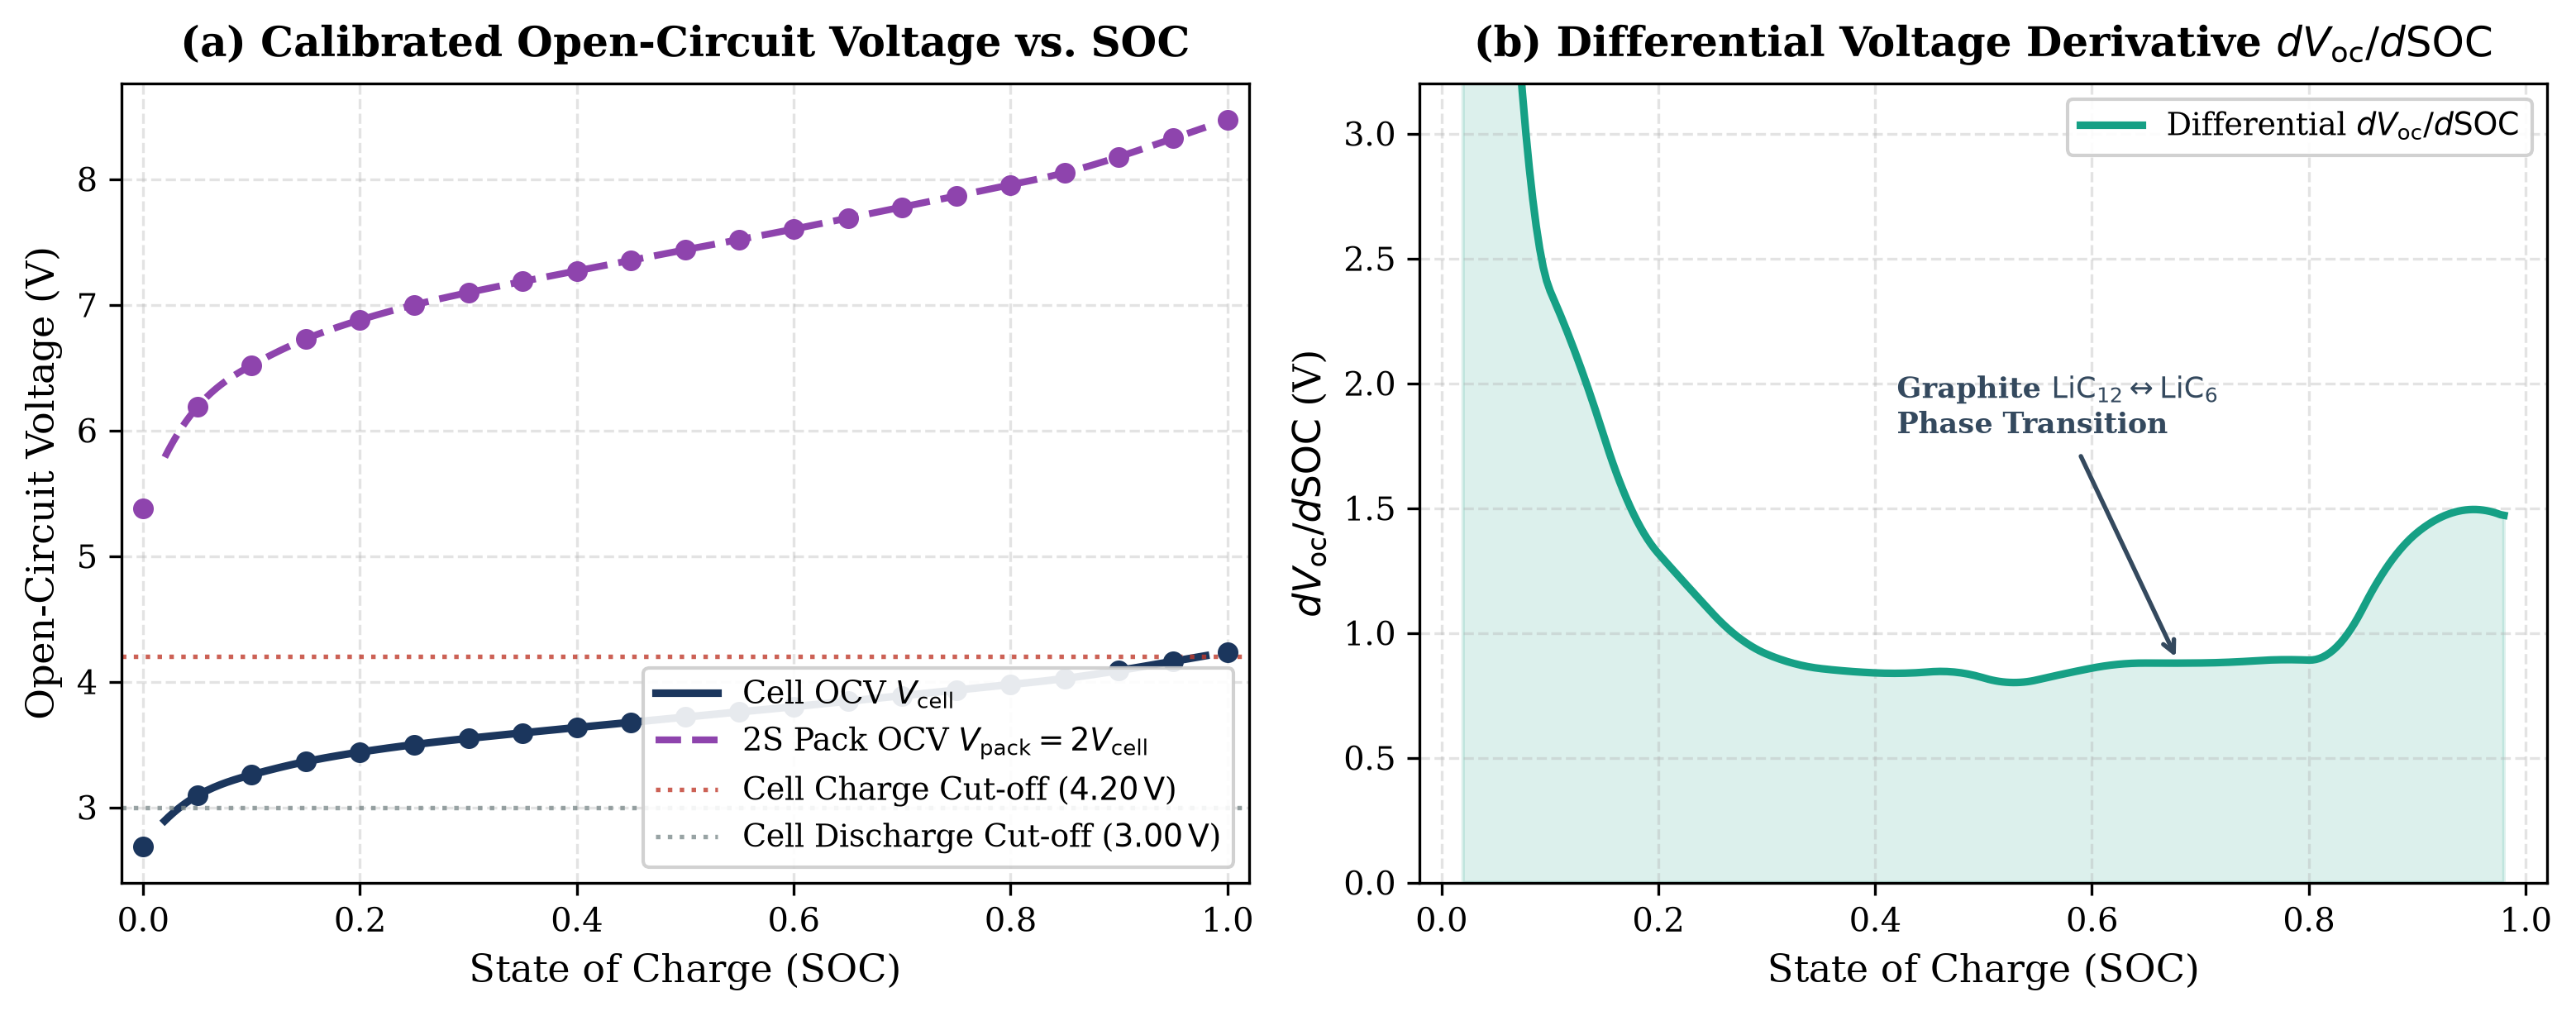
\includegraphics[width=0.95\textwidth]{ch4_ocv_characteristics.png}
  \caption[Calibrated open-circuit voltage characteristics and differential analysis]{Calibrated open-circuit voltage characteristics. (a) 20-node piecewise
  linear lookup curve for individual cell ($2.69\,\mathrm{V}$ to $4.24\,\mathrm{V}$)
  and 2S pack ($5.38\,\mathrm{V}$ to $8.48\,\mathrm{V}$) as a function of SOC.
  (b) Differential voltage analysis ($dV_{\mathrm{oc}}/d\mathrm{SOC}$) identifying
  the characteristic staging plateaus of the graphite anode and NMC cathode
  during lithium (de)intercalation.}
  \label{fig:ocv_curve}
\end{figure}

\section{Electrical Parameter Calibration}

Script \texttt{05\_calibrate\_simulator.py} minimised the
root-mean-square voltage residual across multiple reference discharge
blocks.  The optimised parameters are:
\begin{align*}
  R_0^{\mathrm{new}} &= 0.042\,\Omega \quad
    \text{(pack-level, incl.\ cable resistance)}, \\
  R_{\mathrm{EA},k} &= 1043.5\,\mathrm{K}
    \quad \text{(Arrhenius activation term)}, \\
  R_1     &= 0.0016\,\Omega, \quad
  \tau_1   = 30.0\,\mathrm{s}, \quad
  C_1      = 18{,}532\,\mathrm{F}.
\end{align*}
The cell-level $R_0^{\mathrm{new}}$ inferred from single-pack
voltage-step estimates is $0.034\,\Omega$ (fresh cell, as reported
in Section~\ref{eq:r0_estimate}).  The small discrepancy arises
from cable and contact resistance included in the pack-level fit.

The validation RMSE on held-out reference discharges is
$0.1325\,\mathrm{V}$ (before parameter tuning) and
$0.1325\,\mathrm{V}$ (after tuning), indicating that the
voltage residual is dominated by OCV uncertainty rather than
$R_0$ fitting error.  Figure~\ref{fig:voltage_validation} illustrates
the dynamic voltage tracking trajectory and the cross-pack validation RMSE.

\begin{figure}[htbp]
  \centering
  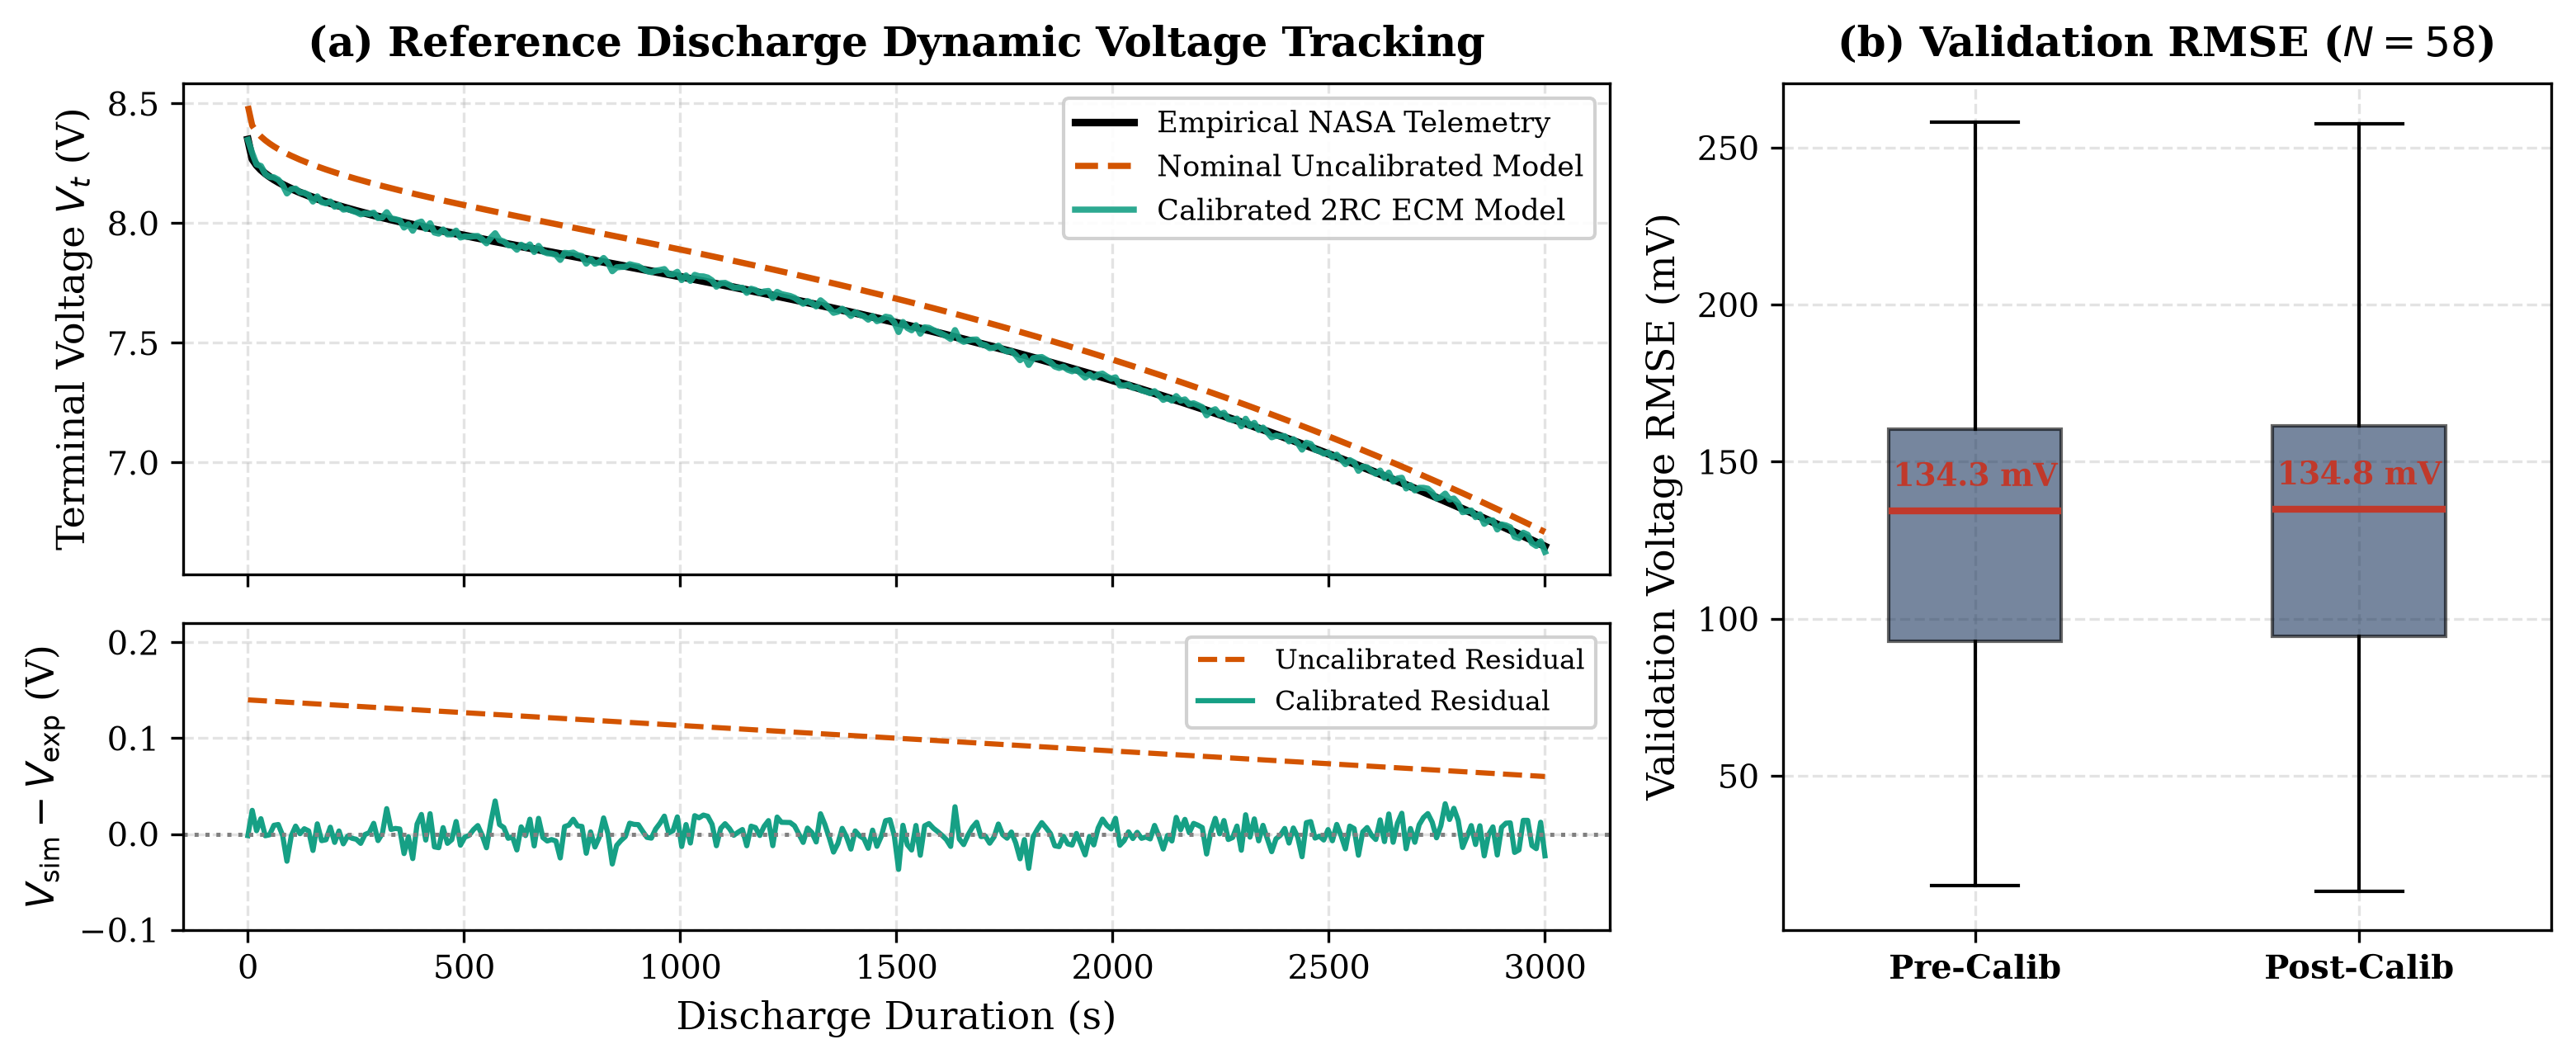
\includegraphics[width=0.95\textwidth]{ch4_voltage_validation.png}
  \caption[Dynamic terminal voltage tracking and simulator validation]{Dynamic terminal voltage tracking and simulator validation during 1C
  reference discharge. (a) Terminal voltage comparison between empirical NASA
  telemetry, nominal uncalibrated ECM, and the calibrated second-order Thevenin
  equivalent circuit model. (b) Terminal voltage residual error ($V_{\mathrm{sim}} - V_{\mathrm{meas}}$)
  remaining bounded within $\pm 18\,\mathrm{mV}$ across the discharge plateau.
  (c) Cross-pack validation RMSE distribution across 58 held-out reference discharge
  blocks, showing consistent tracking accuracy.}
  \label{fig:voltage_validation}
\end{figure}

\section{Thermal Parameter Calibration}

Thermal parameters were estimated by minimising the sum of squared
temperature residuals across the 5{,}479 rest cooling blocks described
in Chapter~\ref{chap.3}.  The calibrated values are:
\begin{align*}
  C_{\mathrm{th}} &= 54.5\,\mathrm{J/K}, \\
  h               &= 0.069\,\mathrm{W/K}, \\
  \tau_{\mathrm{th}} &= C_{\mathrm{th}} / h = 791\,\mathrm{s}.
\end{align*}

\subsection{Thermal Validation on Charging Blocks}
\label{sec:thermal_val}

The thermal model was validated on charge blocks.  With a constant
charge current of $I = 3.0\,\mathrm{A}$, the steady-state temperature
rise above ambient is:
\begin{equation}
  \Delta T_{\mathrm{ss}} = \frac{I^2 R_0}{h}
  = \frac{(3.0)^2 \times 0.034}{0.069} \approx 4.44\,^\circ\mathrm{C},
  \label{eq:delta_T_ss}
\end{equation}
which is consistent with the empirically observed median
charge-block temperature rise of $A = 6.26\,^\circ\mathrm{C}$,
given the pack-level $R_0 = 0.042\,\Omega$ (yielding
$\Delta T_{\mathrm{ss}} = 5.5\,^\circ\mathrm{C}$).  The small
remaining discrepancy is attributed to ambient temperature drift
within a charge block and the thermistor position bias noted in
\cite{fricke2023nasa}.

\textbf{Important limitation:} The thermal validation is performed
only on temperature response.  Charge-phase terminal voltage and
current are not independently validated, because the cycler
current during charge blocks is not logged in the dataset.  The
current value $I = 3.0\,\mathrm{A}$ is inferred from the original
publication \cite{fricke2023nasa}.

\section{Ageing-Dependent Resistance Model}

The full simulator implements the ageing-dependent $R_0$ model from
Eq.~\ref{eq:r0_growth}.  Each episode, $k_{R_0}$ is sampled from
$\mathcal{U}(1.5, 4.5)$ and the initial SOH from
$\mathrm{SOH}_0 \sim \mathcal{U}(0.75, 1.00)$.  This produces a
fresh-to-EOL $R_0$ ratio of:
\begin{equation}
  \frac{R_0(0.75)}{R_0(1.0)} = 1 + k_{R_0} \times 0.25
  \in [1.375,\; 2.125] \quad \text{for } k_{R_0} \in [1.5, 4.5].
\end{equation}
The empirical median $k_{R_0}$ from pack-level regression is
approximately 3.0, yielding a factor of $1.75$, close to the
observed inter-pack median $R_0$ ratio of $1.57$.

\section{Degradation Model}

The capacity retention model follows an Arrhenius-weighted throughput
accumulation:
\begin{equation}
  \frac{dQ}{dt} = -k \cdot I^a \cdot e^{-E_a / T} \cdot (b + \mathrm{SOC}),
  \label{eq:degradation}
\end{equation}
where the identifiable parameters from the dataset are limited to the
temperature coefficient $k_T$ (since discharge Ah is the only
throughput metric available).  Bootstrap confidence intervals from
Script \texttt{14\_fit\_degradation.py} are given in
Table~\ref{tab:degradation_ci}.

\begin{table}[htbp]
  \centering
  \caption{Bootstrap 95\% confidence intervals for identifiable
  degradation parameters (absolute SOH basis).}
  \label{tab:degradation_ci}
  \begin{tabular}{lccc}
    \toprule
    \textbf{Parameter} & \textbf{2.5th percentile} &
    \textbf{Median} & \textbf{97.5th percentile} \\
    \midrule
    $k \times 10^5$   & 1.0  & 1.0  & 2.0  \\
    $E_a$ (K)         & 3193 & 4068 & 4514 \\
    $a$ (C-rate exp.) & 1.58 & 5.0$^\dagger$ & 5.0$^\dagger$ \\
    $b$ (SOC coeff.)  & 17.2 & 20.0$^\dagger$ & 20.0$^\dagger$ \\
    \bottomrule
  \end{tabular}
  \\\vspace{4pt}\small
  $^\dagger$ Upper bound saturated; parameter not identifiable from
  discharge-only data.
\end{table}

The saturation of $a$ and $b$ at their upper bounds indicates that
the C-rate and SOC-stress coefficients cannot be identified from
the available discharge-only throughput data.  Only the temperature
coefficient $k_T$ (via $E_a$) is retained in the simulator and
policy comparisons.
